%************************************************
\chapter{Flash simulation of samples with Normalizing Flows}\label{ch:fs} % $\mathbb{ZNR}$
%************************************************

Having discussed the importance and the challenges of event simulation at LHC, and having described the Deep Learning Normalizing Flows approach, we dedicate this chapter to the practical implementation of an end-to-end sample generator.

\section{Target variables}

As we discussed in Section \ref{sec:targets}, we choose to target the VBF Channel of H$\rightarrow\mu^+\mu^-$. Thanks to the clear signature, we only needed to simulate jets and muons out of all the possible objects in a NanoAOD. 

However, because our Machine Learning Models need proper training data, we needed a well known process, extensively studied at CMS and having already been simulated through FullSim in large numbers. We thus turned to the t$\overline{\text{t}}$ process.

\subsection{The t$\overline{\text{t}}$ process}
The top quark is an important component of the standard model, especially because of
its large mass, and its properties are critical for the overall understanding of the theory. Measurements of the top quark-antiquark pair (t$\overline{\text{t}}$) production cross section test the predictions of
quantum chromodynamics (QCD), constrain QCD parameters, and are sensitive to physics beyond the SM. The t$\overline{\text{t}}$ process is also \emph{the dominant SM background to many searches for new
physical phenomena}, and its precise measurement is essential for claiming new discoveries.
The copious top quark data samples produced at the CERN LHC enable measurements of the t$\overline{\text{t}}$
production rate in extended parts of the phase space, and differentially as a function of the kinematic properties of the t$\overline{\text{t}}$ system. Inclusive and differential cross section measurements from
proton-proton (pp) collisions at centre-of-mass energies of 13 TeV have been reported by
the CMS collaboration in \cite{Sirunyan_2017}.

\graffito{were our samples dijets or mixed?}
Top quarks decay almost exclusively into a W boson and a b quark. The W may then decay in either a q$\overline{\text{q}}$ or a lepton and its corresponding neutrino, ensuring that the events will be well populated with both jets and muons, our simulation targets. Figure \ref{fig:ttfig} shows some details about t$\overline{\text{t}}$ production at LHC.

\begin{figure}
    \centering
    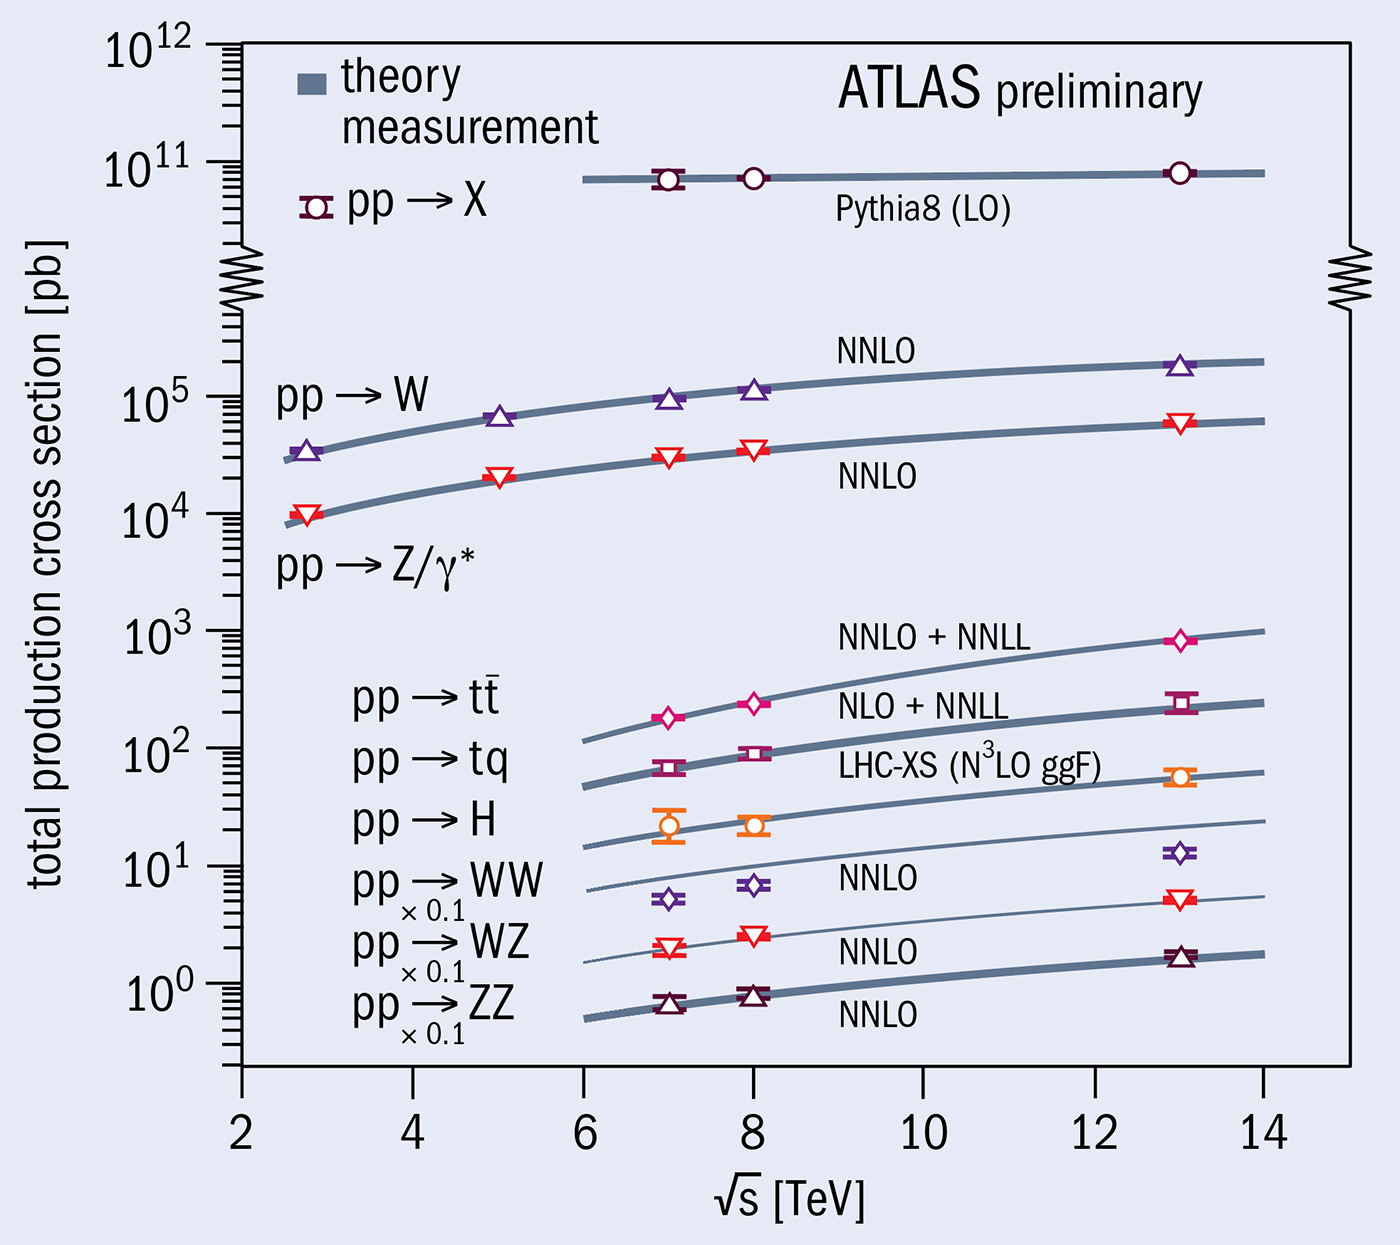
\includegraphics[scale=0.2]{gfx/ch5/CCMarApr_LHC10_fig2.jpg}\quad
    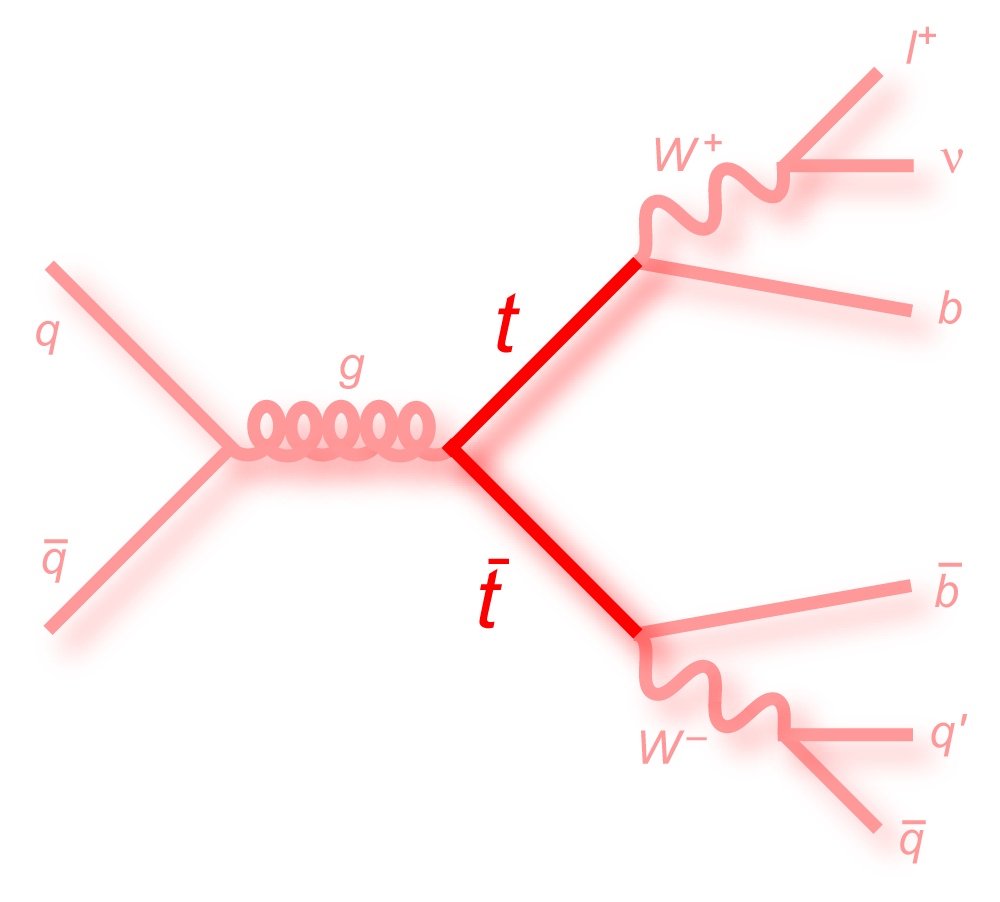
\includegraphics[scale=0.3]{gfx/ch5/feynman_ttbar_ljets_longt.png}
    \caption[t$\overline{\text{t}}$ plots]{Top: The t$\overline{\text{t}}$ process is dominating the cross sections at LHC, making it one of the leading SM background processes. Bottom: the production diagram for proce}
    \label{fig:ttfig}
\end{figure}

Having at our disposal a large set of FullSim MC samples for t$\overline{\text{t}}$ dijet(??) events, we used these to \emph{train} two Normalizing Flows models on the two target objects.
\subsection{Jets}
ref to \cite{nanoaodcont}
\subsection{Muons}

\subsection{Extraction and preprocessing}

\section{Models design}

\subsection{Software and packages}

\subsection{Architectures and trainings}

\section{Results}

\subsection{1d distributions and correlations}

\subsection{Conditioning}

\section{A prototype end-to-end analysis sample generator}
